\documentclass[dvipdfmx,uplatex]{jsarticle}

%% Packages
\usepackage{graphicx,color,hyperref}
\usepackage{algorithm}
\usepackage{algorithmic}
\usepackage{url}
\usepackage{lscape}
\usepackage{mathtools}
\usepackage{here}
\usepackage{amsmath,amssymb,amsfonts}
\usepackage{amsthm}
\usepackage{tikz}
\usepackage{tcolorbox}
\usepackage{pxjahyper}

%% Theorem Styles
\newtheorem{theorem}{定理}
\newtheorem{proposition}{命題}
\newtheorem{cor}{系}
\newtheorem{definition}{定義}
\newtheorem{problem}{問題}
\theoremstyle{remark}
\newtheorem{remark}{注意}
\newtheorem{requirement}{条件}

%% Environment (Colorful Box)
\newenvironment{simplebox}{
    \begin{tcolorbox}[
        fonttitle=\bfseries,
    ]
}{
    \end{tcolorbox}
}

\newenvironment{method}[1]{
    \begin{tcolorbox}[
        colframe=green!50!black,
        colback=green!50!black!10!white,
        colbacktitle=green!50!black!40!white,
        coltitle=black,
        fonttitle=\bfseries,
        title={#1}
    ]
}{
    \end{tcolorbox}
}

\newenvironment{experiment}[1]{
    \begin{tcolorbox}[
        colframe=violet,
        colback=violet!10!white,
        colbacktitle=violet!40!white,
        coltitle=black,
        fonttitle=\bfseries,
        title={#1}
    ]
}{
    \end{tcolorbox}
}

\newenvironment{kansou}{
    \begin{tcolorbox}[
        colframe=brown,
        colback=brown!10!white,
        colbacktitle=brown!40!white,
        coltitle=black,fonttitle=\bfseries
    ]
}{
    \end{tcolorbox}
}

%% Title
\title{Making Cache Monotonic and Consistent}
\author{\empty}
\date{\empty}

%% Document body
\begin{document}
\maketitle

\begin{itemize}
    \item Link: \url{https://dl.acm.org/doi/10.14778/3574245.3574271}
    \item Conference:
    \item Citation: \cite{cache-consistent}
    \item pdf: \url{https://www.vldb.org/pvldb/vol16/p891-cao.pdf}
\end{itemize}

%% 単調性って何?一貫性って何?

\section{概要}
\begin{simplebox}
\begin{itemize}
    \item キャッシュ置換ポリシーはこれまで様々提案されてきたが、以下の単調性まで考慮して性能評価したものはなかった(キャッシュヒットするが不整合なので結局データベースへのアクセスが発生するという形で処理されていた).
    \begin{itemize}
        \item 整合性: アプリケーションがある時点でのデータベースの一貫したビューを常に観測できること
        \item 単調性: 一度観測した書き込みが失われることがないということ
    \end{itemize}
    \item 本研究では上二つの性質と従来から考慮されてきたキャッシュオーバーフローを統合的に考慮するキャッシュポリシー(MCCPolicy)を提案する.
    \item さらに、MCCPolicyを実用化するためのツールMCCacheを開発した. これは、RedisやMemcachedといった既存のキャッシュシステムに対して導入可能であり、HBase上でのスループットを平均で77.15\%向上させる.
\end{itemize}
\end{simplebox}

\section{背景}
\begin{simplebox}
\begin{itemize}
    \item データベース: $D = \{d_1, d_2, \dots, d_n\}$というデータの集合とする
    \item 書き込み: $W[d_i]$ はデータ$D$の要素$d_i$に対する書き込みを表す.
    \item 読み込み: $R[d_i]$ はデータ$D$の要素$d_i$に対する読み込みを表す.
    \item 書き込みによりデータベースの新しいversionが作られるとする. $D[i]$をversion $i$のデータベースとする. $d[j]$をversion $j$のアイテム$d$の値とする.
\end{itemize}
\end{simplebox}

\section{手法}
\begin{method}{MCC Policy}
\begin{itemize}
    \item リクエスト: $R = \{d_1, d_2, \dots, d_m\}$は複数のデータを同時に読み込むものとする, 書き込みも同様に複数のデータを同時に書き込むものとする.
    \item Consistency(整合性): $R = \{d_1, d_2, \dots, d_m\}$がConsistencyをもつとは、あるversion$l$が存在してて、$R$のすべての要素$d_i$がversion$l$に存在することを意味する. (直感的にはあるバージョンのデータベースしか観測することができないことを意味する.)
    \item Monotonicity(単調性): $R$が$R^\prime$を先行するとは、$R$と$R^\prime$のいずれにも登場するどんなクエリ$d$に対しても、$d$が$R$を読んだとき$d[i]$, $R^\prime$を読んだとき$d[j]$とすると、$i \leq j$が成立することをいう. $R_1, R_2, \dots, R_m$が読み込みリクエストの列とすると, $R_i$が単調であるとは任意の$R_l (l < i)$に対して, $R_l$が$R_i$を先行することをいう. (直感的にはある時点でデータを見たとすると、それより古いバージョンのデータはそのあとには読みださないということを意味する.)
    \item 上の定義から読み出しリクエストには次の三つの可能性がある.
    \begin{itemize}
        \item Monotonic consistent cache hit (MCC hit): $R$に含まれるすべてのデータがキャッシュに存在し、consistentかつmonotonicでありかつ、読み出しリクエストに含まれるデータのバージョンが十分に新しいこと.
        \item Non-MCC hit: $R$に含まれるすべてのデータがキャッシュに存在するが、MCC hitではないこと.
        \item Cache miss: $R$に含まれるデータの一部がキャッシュに存在しないこと.
    \end{itemize}
    \item これまではcache missとconsistencyは別に考慮されていた、すなわちどのデータをevictするかをcache policyが決定し、consistentでない場合にはアプリケーション側でリフェッチすることで対応していた.
    \item MCC policy: 通常のキャッシュポリシー(キャッシュがいっぱいになったら、どのデータをevictするかを決める)に加えて、non-MCCなhitを防ぐためにアイテムの更新を行うようなキャッシュ戦略.
    \item Version戦略: MCC hitのときにどのバージョンに一致させるかは選択の余地がある.
    \begin{itemize}
        \item Eager: つねに最も新しいバージョンを選択する.
        \item Lazy: リクエストをMCC hitにできる、できるだけ古いバージョンを選択する.
    \end{itemize}
    \item 三つのモデルを考える.
    \begin{itemize}
        \item Batch: すべての読み込み、書き込み列は事前に知られている.
        \item Semi-online: 読み込みリクエストは事前に知られているが、書き込みは知られていない.
        \item Online: すべての読み込み、書き込み列は未知.
    \end{itemize}
\end{itemize}
\end{method}

\begin{method}{複雑性と特徴づけ}
\begin{itemize}
    \item 問題定義(MCC Problem)
    \begin{itemize}
        \item 入力: サイズ$k$のキャッシュ、書き出し読み込みリクエスト列$\ell$とstaleness bound$s$.
        \item 出力: キャッシュ$C$上での$\ell$用のMCCスケジュール$P$
        \item 目的: データベース$D$からの取得回数を最小化
    \end{itemize}
    \item 計算複雑性
    \begin{itemize}
        \item MCC ProblemはEager戦略ではNP-hardである.
        \item MCC ProblemはLazy戦略ではPに属する.
    \end{itemize}
    \item 特徴づけ: MCC Problemの難しさの原因を調べる.
    \begin{itemize}
        \item Obsolete items: あるリクエスト列$\ell$を考える. ある時点でキャッシュにあるアイテム$d$がobsoleteであるとは、それよりあとのどんな読み込みリクエスト$R$に対しても、$d$がどんなMCCスケジュールにおいても$R$に答えるのに必要ないことをいう.
        \item 方針: キャッシュオーバーフローがおきたら、obsoleteなアイテムから削除していく.
        \item (1): 毎回のリクエストのあとにobsoleteなアイテムを削除すると、non-MCC hitsを無くすことができる.
        \item (2): Lazy戦略においてobsoleteなアイテムかどうかを決定することは多項式時間でできる、Eager戦略においてはcoNP-completeな問題となる.
    \end{itemize}
    \item すなわち、難しさは本質的にはobsoleteなアイテムを決定することにある.
\end{itemize}
\end{method}

\begin{figure}
    \centering
    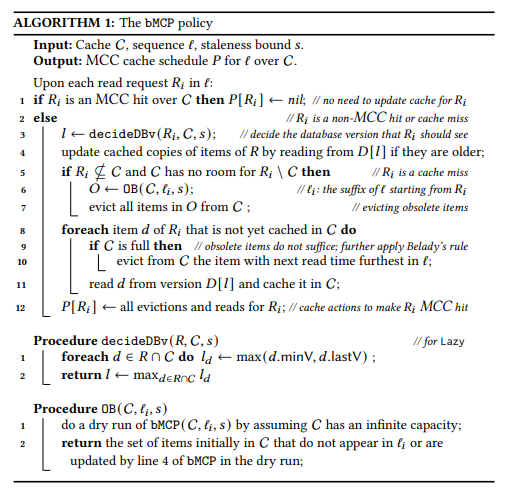
\includegraphics[width=0.6\textwidth]{img/cache-consistent/batch.png}
    \caption{Batch MCC Policyのアルゴリズム}
    \label{fig:batch-algorithm}
\end{figure}

\begin{method}{Batch MCC Policy}
\begin{itemize}
    \item Batch設定において、Lazy戦略でもEager戦略でも動作するMCC policy: bMCPを示す. この戦略はLazy戦略においては最適性が示されている.
    \item bMCPのアルゴリズムは以下の通り
    \begin{itemize}
        \item $R$がMCC hitなら終わり.
        \item non-MCC hitもしくはmissならば一致させるバージョンを決定する.
        \item $R$に含まれるデータでキャッシュにあるものは、バージョンと一致しないものを取得.
        \item $R$に答えるのに必要な項目がキャッシュに存在しない場合は以下の操作を行う.
        \begin{itemize}
            \item obsoleteな項目をすべて削除
            \item $R$に含まれるがキャッシュに存在しない項目をすべて削除
        \end{itemize}
        \item キャッシュに空きがない場合はBeladyのルールを適用する.
    \end{itemize}
    \item データベースバージョンの決定
    \begin{itemize}
        \item Eager: 最新
        \item Lazy: キャッシュ内のデータ$x$について、以下のバージョンを記録しておく.
        \begin{itemize}
            \item $x.minV$: $x$を含む最小のデータベースバージョン
            \item $x.lastV$: 現在のリクエストより前のリクエストが最後に使用した$x$と同じバージョンを持つ最小のデータベースバージョン
            \item $R$に含まれて、かつキャッシュ$C$に存在するデータ$x$についての$max(x.minV, x.lastV)$の最大値
        \end{itemize}
    \end{itemize}
    \item obsolete itemsの特定
    \begin{itemize}
        \item キャッシュ$C$が無限の要領を持つと仮定して、dry-runすることでobsoleteなアイテムを特定する.
    \end{itemize}
    \item このアルゴリズムは多項式時間アルゴリズムであり、Lazy戦略においては最適であることが示されている.
\end{itemize}
\end{method}

\begin{method}{Online MCC Policy}
\begin{itemize}
    \item sMCP: Semi-online MCC Policy
    \begin{itemize}
        \item obsoleteなアイテムの特定がsemi-onlineでは不可能なため、obsoleteかどうかを判定する機械学習モデルを用いる, このポリシーをsMCPと呼ぶ.
        \item Competitiveness: ポリシー$P$がポリシー$P^\prime$に対して$c$-competitveであるとは $\mathrm{cost}(P,l) \leq c\cdot \mathrm{cost}(P^\prime,l) + O(1)$ であることをいう.
        \item $\epsilon(M) = \eta(l)/\mathrm{cost}(\mathrm{OPT}, l)$と定義する.
        \item $\mathrm{CR}(sMCP)$をsMCPの最適なポリシー$\mathrm{OPT}$に対するcompetitive ratioとする.
        \item すると$\mathrm{CR}(sMCP) \leq 1 + \epsilon(M)$である.
        \item sMCP${}^*$をsMCPとbMCP${}^0$(bMCPからobsoleteなアイテムを取り除く操作を無くしたもの)を組み合わせたものとすると, sMCP${}^*$は$18$-competitiveでML-robustとなる.
    \end{itemize}
    \item oMCP: Online MCC Policy
    \begin{itemize}
        \item sMCPの制約に加えて、Beladyのルールを利用してキャッシュ内のアイテムを削除することもできない.
        \item そのためBeladyのルールを使って削除している部分はLRUで削除する.
    \end{itemize}
\end{itemize}
\end{method}

\section{実験結果}
\begin{experiment}{実験手法}
\begin{itemize}
    \item データセット
    \begin{itemize}
        \item YCSBで生成されたデータ
        \item Real-life traces: Wiki, Twitter, Ibm
    \end{itemize}
    \item キャッシュポリシー
    \begin{itemize}
        \item bMCP, sMCP, oMCP
        \item mcBelady (bMCPからobsolete itemの削除を行わなかったバージョン), LRU, LRU-k, BeladySet, LRUSet
    \end{itemize}
    \item システム
    \begin{itemize}
        \item Redis, Memcached, HBaseの四つにポリシーを実装.
    \end{itemize}
\end{itemize}
\end{experiment}

\begin{figure}
    \centering
    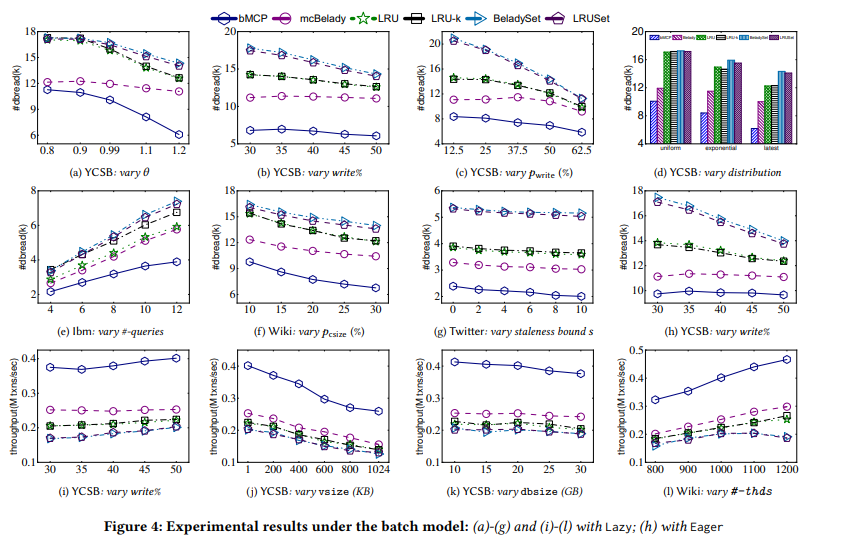
\includegraphics[width=0.7\textwidth]{img/cache-consistent/experiment-result.png}
    \caption{実験結果}
    \label{fig:experiment-result}
\end{figure}

\begin{experiment}{実験結果}
\begin{itemize}
    \item データベースの読み込み回数のコスト評価
    \begin{itemize}
        \item bMCPではDBの読み込み回数が基本的にほかのどのポリシーよりも小さい(表\ref{fig:experiment-result})
    \end{itemize}
    \item セミオンラインモデル、オンラインモデルにおける効果とML耐性
    \begin{itemize}
        \item MLモデルの精度を変更して実験.
        \item 表\ref{fig:semionline-online}より精度が高いときは性能有意であり、精度が低くてもある程度までは優位. しかし精度が75\%以下になると劣化することもある.
    \end{itemize}
    \item スループット評価
    \begin{itemize}
        \item lightgbmを分類器として用いてスループットを検証.
        \item 結果は表\ref{fig:experiment-result}に示すが, bMCPはほかのポリシーよりスループットが大きい.
        \begin{itemize}
            \item YCSB: mcBelady, LRU-k, LRU, BeladySet, 
LRUSetそれぞれで52.80\%, 80.81\%, 79.06\%, 109.82\%
107.97\%早くなった.
        \end{itemize}
        \item sMCP, oMCPもモデル精度が高いため、スループットが高い.
    \end{itemize}
\end{itemize}
\end{experiment}

\begin{figure}
    \centering
    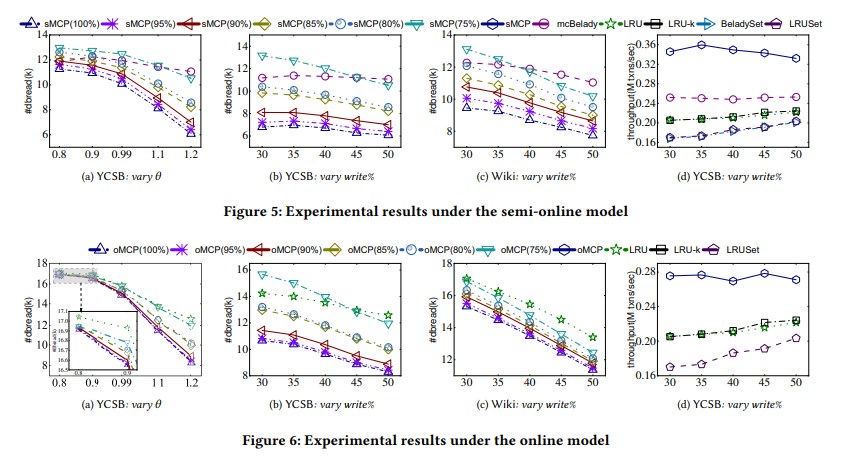
\includegraphics[width=0.7\textwidth]{img/cache-consistent/semionline-online.png}
    \caption{実験結果}
    \label{fig:semionline-online}
\end{figure}

\section{感想}
\begin{kansou}
\begin{itemize}
  \item キャッシュポリシーについての論文初めて読んだ.
  \item キャッシュの一貫性とか単調性については確かにこれは必要だと思った.
  \item オンラインで機械学習モデル使ってもスループットが上がるのは面白い.
\end{itemize}
\end{kansou}

\bibliographystyle{jplain}
\bibliography{template.bib}

\end{document}